% Costello thesis + costello pairings for beginners+ lynnpairing2007
\section{Miller's algorithm for the Weil and Tate pairings}
\label{sec:ch2.weilandtatepairings}

In the current chapter we review the theoretical foundations of Weil and Tate  pairings with regards to Miller's algorithm on how to compute them. The theoretical introductions (refer to \refSubsection{secs:ch2.theoreticweil} and \refSubsection{secs:ch2.theoretictate}) use a more generalized notations based on \cite{lynn2007implementation}. The practical examples presented later in the chapter (refer \ref{ssec:ch2.weilpairing} and \refSubsection{ssec:ch2.tatepairing}) are motivated by \cite{theory.pairings.for.beginners}, therefore we will restrict the analogues notations to be aligned with \cite{theory.pairings.for.beginners}.  We note that the definitions in our context are apply to elliptic curves over finite fields, but the more general definitions are analogous, see \cite{Sil09, Gal05} for more detail.

\subsection{Theoretic overview of Weil Pairing}
\label{secs:ch2.theoreticweil}

Let $E$ be an elliptic curve containing $n$ points over a field $\mathbb{F}_q$. Let $G$ be a cyclic subgroup of $E(\mathbb{F}_q)$ of order $r$ with $r, q$ coprime. Let $k$ be the smallest positive integer such that $E(\mathbb{F}_{q^k})$ contains all of $E[r]$. 

We define the Weil pairing $f : E[r] \times E[r] \to \mathbb{F}_{q^k}$ as follows. For a pair of points $P, Q \in E[r]$, choose any $R, S \in E(\mathbb{F}_{q^k})$ such that $S \neq R, P+R, P+R-Q, R-Q$. Let $f_P$ be a rational function with divisor $(f_P) = (P+R)^r/(R)^r$, (In other words we have $r$ zeroes at $P+R$ and $r$ poles at $R$.  In standard notation this is $r\langle P+R \rangle - r\langle R \rangle$.) and similarly let $f_Q$ be a rational function with divisor $(f_Q) = (Q+S)^r/(S)^r$, then

\insertEquationEnvironmentWithLabel{
f(P, Q) = \frac{f_P(Q+S)/f_P(S)}{f_Q(P+R)/f_Q(R)}}{eq:frationalpqweil}

%%% <- ez ezert lenyeges, mert nem lett ebbe a szovegbe beleemelve, de genus > 1 esetben mar figyelembe kellene venni az intermediat zero es pole-okat is 

It can be shown that the value in \refEquation{eq:frationalpqweil} is independent of the choices for $R, S$. The conditions for choosing $R, S$ ensure we never evaluate $f_P$ nor $f_Q$ at a zero or pole. Also both $f_P, f_Q$ are only unique up to a constant, but this has no effect on the final answer since quotients of these functions are computed and the constants cancel out. Refer \refDef{def:weilpairingproperties} in \textit{Appendix \refSubsection{apx_theory__pairing_properties_weil}} for more information regarding the provable properties of Weil pairing. 

We note that finding explicit expressions for these functions is infeasible for cryptographically useful pairings, hence we will use Miller's algorithm \cite{Miller1986, Miller04} instead, that evaluates these functions in at the required points. His algorithm resembles a typical exponentiation routine that performs square and multiply as we continues in the subsequent \refSubsection{sssec:ch3.millersalgorithmforweilpairing}

\subsubsection{Miller's algorithm for the Weil pairing}
\label{sssec:ch3.millersalgorithmforweilpairing}

For the Weil pairing we need to evaluate some rational function $f_P$ with divisor $(P+R)^r/(R)^r$.  For any points $U, V$, let $L_{U,V}(X, Y)$ be an equation for a line through $U$ and $V$, let $T_U(X, Y)$ be an equation for the tangent through $U$, let $V_U(X, Y)$ be an equation for a vertical line through $U$ (e.g.\ $X - x$, where $U = (x, y)$).

Since $T_U = L_{U,U}$ and $V_U = L_{U,-U}$, defining $T_U$ and $V_U$ is unnecessary but they aid comprehension. Note if $U = -U$ then $T_U$ is the same as $V_U$.

For an integer $k$, let $f_k$ be a rational function with divisor
$(f_k) = \frac{(P+R)^k}{(R)^k(kP)}.$ Observe $f_r = f_P$, since $rR = O$. It can be checked that $
\left( f_a \cdot f_b \cdot \frac{L_{aP,bP}}{V_{(a+b)P}}\right) = (f_{a+b})
$ ,with computation on the divisors: 
$$\frac{(P+R)^a}{(R)^a(aP)} \cdot \frac{(P+R)^b}{(R)^b(bP)} \cdot \frac{(aP)(bP)(-(a+b)P)}{(a+b)P(-(a+b)P)} = \frac{(P+R)^{a+b}}{(R)^{a+b}((a+b)P)}.$$

Which yields us with the formula:  $f_k^2 \cdot \frac{T_{kP}}{V_{2kP}} = (f_{2k})$.  Thus we may compute $f_P(Q) = f_r(Q)$ using \textit{Algorithm \ref{alg:milleralgweiltheory}} where the binary representation of $r$ is $r_t \ldots r_0$.

%%%% Algorithm
\begin{algorithm}
	\label{alg:milleralgweiltheory}
	\caption{Miller's algorithm for Weil pairing \cite{lynnpairing2007}. $x = f_P(Q)$}
	\KwIn{Binary representation of $r$ is $r_t \ldots r_0$}
	\KwOut{$x = f_P(Q)$}
	$x_1 \leftarrow V_{P+R}(Q) / L_{P,R}(Q)$\;
	$x \leftarrow x_1$\;
	$Z \leftarrow P$\;
	\For{$i = t-1$ \KwTo $0$}{
		$x \leftarrow x^2 \cdot T_Z(Q) / V_{2Z}(Q)$\;
		$Z \leftarrow 2Z$\;
		\If{$r_i = 1$}{
			$x \leftarrow x \cdot x_1 \cdot L_{Z,P}(Q) / V_{Z+P}(Q)$\;
			$Z \leftarrow Z + P$\;
		}
	}
	\Return $x$\;
\end{algorithm}
%%%%

On termination, we have $x = f_P(Q)$ (and $Z = rP = O$). Throughout the algorithm we may multiply the equation of any line $L$, $T$, $V$ by an arbitrary constant, thus this algorithm really computes $f_P(Q)$ for one possible choice of $f_P$.

\subsection{Theoretic overview of Tate Pairing}
\label{secs:ch2.theoretictate}

We now consider the Tate pairing. Recall we wish to compute $f_P(Q)$ where $f_P$ has divisor $(P)^r$. We can view our current situation as a special case of the above with $R = O$. Thus define the intermediate functions $f_k$ by $(f_k) = (P)^k/(kP)$.

We have $(f_r) = (f_P)$. The following identities can be obtained by simplifying earlier formulas using $R = O$, but it is easy enough to check them directly.

For example, we can show $(f_k) = \left( \displaystyle\prod_{i=1}^{k-1} \frac{L_{iP}}{V_{(i+1)P}}\right)$ via
$$(f_k) = \frac{(P)(P)}{(2P)} \cdot \frac{(P)(2P)}{(3P)} \cdots \frac{(P)((k-1)P)}{(kP)}.$$
We could compute $f_r(Q)$ using this formula, but this is clearly impractical for large $r$.

\subsubsection{Miller's algorithm for the Tate pairing}
\label{sssec:ch3.millersalgorithmfortatepairing}

In \cite{lynnpairing2007} is found that 
$(f_{2k}) = \left(f_k^2 \cdot T_{kP} / V_{2kP}\right)$
which can be shown with direct calculation:
$$\frac{(P)^{2k}}{(2kP)} = \frac{(P)^{2k}}{(kP)^2} \cdot \frac{(kP)^2(-(2kP))}{(2kP)(-(2kP))}$$
and similarly it can be shown
$(f_{k+1}) = (f_k \cdot L_{kP,P} / V_{(k+1)P}).$
Thus leading us to the following \textit{\ref{alg:milleralgorithmtate} Algorithm} that computes $f_P(Q)$ given points $P, Q$ (where $P$ has order $r$). Let the binary representation of $r$ be $r_t \ldots r_0$.


\begin{algorithm}
	\label{alg:milleralgorithmtate}
	\caption{Miller's algorithm for Tate pairing. $x = f_P(Q)$}
	\KwIn{Binary representation of $r$ is $r_t \ldots r_0$}
	\KwOut{$x = f_P(Q)$}
	$x \leftarrow 1$\;
	$Z \leftarrow P$\;
	\For{$i = t-1$ \KwTo $0$}{
		$x \leftarrow x^2 \cdot T_Z(Q) / V_{2Z}(Q)$\;
		$Z \leftarrow 2Z$\;
		\If{$r_i = 1$}{
			$x \leftarrow x \cdot L_{Z,P}(Q) / V_{Z+P}(Q)$\;
			$Z \leftarrow Z + P$\;
		}
	}
	\Return $x$\;
\end{algorithm}

When the algorithm finishes we have $x = f_r(Q)$ (and $Z = rP = O$). Note this algorithm can be viewed as the previous \textit{Algorithm \ref{alg:milleralgweiltheory}} with $x_1 = 1$.

Building upon \ref{secs:ch2.theoreticweil}, \refSubsection{secs:ch2.theoretictate} and the introduced definitions from \refSection{sec:ch1.divisiors} we examine further in \refSubsection{ssec:weilandtatepairingpractice} how the Weil and Tate pairing may be used in a practical setting trough examples motivated by \cite{theory.pairings.for.beginners}. 

\section{Merging the Theory with Practice}
\label{ssec:weilandtatepairingpractice}

First of all, in this section we will use the notation $w_r(P, Q)$
for the (order $r$) Weil pairing of $P$ and $Q$ and $t_r(P, Q)$ for their
(order $r$) Tate pairing, as this will help when discussing differences and
relationships between them.  However after this section, it will be distinguishable 
 which pairing we mean and what the value of $r$ is (the largest prime
factor of $\#E(\mathbb{F}_q)$), thus we will return to the notation most
commonly seen in the literature by simply write $e(P, Q)$.


Both pairings make use of a special case of the following fact we recall from \refSection{sec:ch1.divisiors}: a divisor $D = \sum_P n_P(P)$ is principal (i.e.\ the divisor of a
function) if and only if $\sum_P n_P = 0$ and $\sum_P [n_P]P = \BigO$
on $E$. For any $m \in \mathbb{Z}$ and $P \in E$, it follows that there exists
a function $f_{m,P}$ with divisor
\begin{equation}\label{eq:miller-divisor}
	(f_{m,P}) = m(P) - ([m]P) - (m-1)(\BigO),
\end{equation}
where we note that for $m = 0$, one can take $f_{0,P} = 1$ with $(f_{0,P})$
the zero divisor.

Thus, if $P \in E[r]$, then $f_{r,P}$ has divisor
\begin{equation}\label{eq:torsion-divisor}
	(f_{r,P}) = r(P) - r(\BigO).
\end{equation}
It can be observed that $(f_{m+1,P}) - (f_{m,P}) = (P) + ([m]P) - ([m+1]P) -
(\BigO)$, which is exactly the divisor of the function
$\ell_{[m]P,\,P} / v_{[m+1]P}$, where $\ell_{[m]P,\,P}$ and $v_{[m+1]P}$
are the sloped and vertical lines used in the chord-and-tangent addition of the
point $[m]P$ and $P$ (see Figure~5.1). This means we can build $f_{m+1,P}$
from $f_{m,P}$ via
\begin{equation}\label{eq:miller-step}
	f_{m+1,P} = f_{m,P} \cdot \frac{\ell_{[m]P,\,P}}{v_{[m+1]P}}.
\end{equation}


\begin{figure}[h]
	\centering
	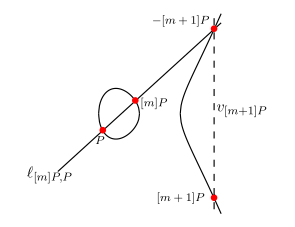
\includegraphics[width=0.5\linewidth]{98_Pictures/Chapter_03/function_divisor}
	\caption{Geometrical interpretation of:$ \left(\frac{\ell_{[m]P,\,P}}{v_{[m+1]P}}\right) = (\ell_{[m]P,P}) - (v_{[m+1]P}) = (P) + ([m]P) - ([m+1]P) - (\BigO)$.}
	\label{fig:functiondivisor}
\end{figure}

%\todo{Example 5.0.1 beepitheto !}

%%%%%%%

\subsection{Miller's Algorithm for Weil and Tate pairing}
\label{ch3:millersalgorithm}

%We briefly recap the pairing definitions from the previous \ref{ssec:ch2.weilpairing}, \refSubsection{ssec:ch2.tatepairing}. For the $r$-torsion points $P$ and $Q$, the Weil and Tate pairings are respectively computed as $\dfrac{f_{r,P}(D_Q)}{f_{r,Q}(D_P)}$ and $f_{r,P}(D_Q)^{(q^k-1)/r}$, where the divisors $D_P$ and $D_Q$ are chosen such that their supports are disjoint from the supports of $(f_{r,Q})$ and $(f_{r,P})$ respectively.

In practical cryptographic application $r$ will be huge, thus for any points $P$ and $Q$ belonging to distinct subgroups in $E[r]$, and since $f_{r,P}$ is a function of degree approximately $r$, computing this function as we did in \refEquation{eq:frationalpqweil} is impossible. In this subsection we describe Miller's algorithm\cite{Miller04}, which makes this computation feasible.

Following \refEquation{eq:miller-divisor}, the divisor $(f_{m,P}) = m(P) - ([m]P) - (m-1)(\BigO)$ can be updated to the divisor $(f_{m+1}) = (m+1)(P) - ([m+1]P) - m(\BigO)$ by adding the divisor $(l_{[m]P,P}/v_{[m+1]P}) = (P) + ([m]P) - ([m+1]P) - (\BigO)$.  This corresponds to the multiplication of functions $f_{m+1} = f_m \cdot l_{[m]P,P}/v_{[m+1]P}$. 

Starting with $f_{2,P} = 2(P) - ([2]P) - (\BigO)$ then, we can repeat this process roughly $r-1$ times to obtain the desired function $f_{r,P} = r(P) - ([r]P) - (r-1)(\BigO) = r(P) - r(\BigO)$. We note that for the last step, when $m = r-1$ we will have $f_{r-1,P} = (r-1)(P) - ([r-1]P) - (r-2)(\BigO)$. Therefore the required divisor is $(P) + ([r-1]P) - 2(\BigO)$ which corresponds to  the vertical line $v_{[r-1]P} = v_{-P} = v_P$. We note that this is the same vertical line that appears on the denominator of $l_{[r-2]P,P}/v_{[r-1]P}$, yielding us with the pairing evaluation function $f_{r,P}$ as the product (\refEquation{eq:fisthepairingproduct}) :
%%% INFO <- corresponds to vertical line is multiplication...

\insertEquationEnvironmentWithLabel{f_{r,P} = l_{[r-2]P,\,P} \cdot \prod_{i=1}^{r-3} \frac{l_{[i]P,\,P}}{v_{[i+1]P}}}{eq:fisthepairingproduct}

The first four sloped lines $l_{[i]P,P}$ and corresponding vertical lines $v_{[i+1]P}$ from the numerator and denominator of the product in \refEquation{eq:fisthepairingproduct} are depicted in \refFigure{fig:milleralgorithmgeometricalrepresentation}. As can be followed, the product (\refEquation{eq:fisthepairingproduct}) is built up incrementally by absorbing each of the $v_{[m+1]P}$ and $f_{m,P}$ to increment into $f_{m+1,P}$, eventually arriving at $f_{r,P}$. Alternatively, it can help to see the divisor sum written out in full, to see the contributions of each of the functions $v_{[i+1]P}$ in the product all at once.


\begin{figure}[h]
	\centering
	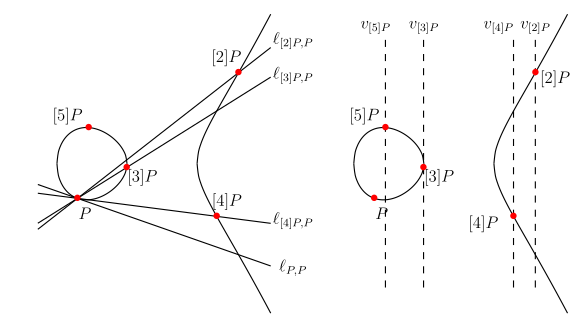
\includegraphics[width=0.7\linewidth]{98_Pictures/Chapter_03/milleralgorithmgeometricalrepresentation}
	\caption{One the left, we can view the first four sloped lines, while on there are the first four vertical lines as arising from the product in \refEquation{eq:fisthepairingproduct}.\cite{theory.pairings.for.beginners}}
	\label{fig:milleralgorithmgeometricalrepresentation}
\end{figure}

\[
\begin{array}{rl}
	l_{P,P}/v_{[2]P}: & (P) + (P) - ([2]P) - (\BigO) \\
	l_{[2]P,P}/v_{[3]P}: & (P) + ([2]P) - ([3]P) - (\BigO) \\
	l_{[3]P,P}/v_{[4]P}: & (P) + ([3]P) - ([4]P) - (\BigO) \\
	& \vdots \\
	l_{[r-4]P,P}/v_{[r-3]P}: & (P) + ([r-4]P) - ([r-3]P) - (\BigO) \\
	l_{[r-3]P,P}/v_{[r-2]P}: & (P) + ([r-3]P) - ([r-2]P) - (\BigO) \\
	l_{[r-2]P,P}: & (P) + ([r-2]P) + (-[r-1]P) - 3(\BigO)
\end{array}
\]

When summing all of the above divisors, most of the inner terms cancel out with one another to leave $(r-1)(P) + (-[r-1]P) - r(\BigO)$, and since $[r-1]P = -P$, we get the divisor of the product being $r(P) - r(\BigO)$.

Roughly speaking, $f_{r,P} = g(x,y)/h(x,y)$, where $g$ and $h$ are degree $r$ functions on $E$. The above method computes $f_{r,P}$ by increasing the degrees of $g$ and $h$ by one each time $f_{m,P}$ is incremented. 

%This is the exact reason when $r$ is exponentially large, the naive method has exponential complexity. Miller's algorithm overcomes this through the following observation.

The function $f_{m,P}$ has $m$ zeros at $P$ and $(m-1)$ poles at $\BigO$. Rather than adding one zero and one pole via multiplying $f_{m,P}$ by linear functions, we can double the number of zeros at $P$ and the number of poles at $\BigO$ if we instead square $f_{m,P}$. Observe that since $(f_{m,P}) = m(P) - ([m]P) - (m-1)(\BigO)$, then
\[
(f_{m,P}^2) = 2m(P) - 2([m]P) - 2(m-1)(\BigO),
\]
which is almost the same as $f_{2m,P}$, whose divisor is
\[
(f_{2m,P}) = 2m(P) - ([2m]P) - (2m-1)(\BigO);
\]
the difference between the two divisors being $(f_{2m,P}) - (f_{m,P}^2) = 2([m]P) - ([2m]P) - (\BigO)$, which corresponds to a function with two zeros at $[m]P$, a pole at $[2m]P$ and another pole at $\BigO$. The function represents the quotient of the tangent line at $[m]P$ and the vertical line at $[2m]P$ -- the lines used to double the point $[m]P$. Thus, we can advance from $f_{m,P}$ to $f_{2m,P}$ via
\[
f_{2m,P} = f_{m,P}^2 \cdot \frac{l_{[m]P,[m]P}}{v_{[2m]P}}.
\]

%%%
%We depict the jump from $f_{m,P}$ to $f_{2m,P}$ (as opposed to the naive method of progressing one-by-one) below.
%
%\todo{Tikz-cd environment + diagram}
%\[
%\begin{tikzcd}[column sep=large]
%	f_{m,P} \arrow[r, "\cdot\frac{l_{[m]P,P}}{v_{[m+1]P}}"] & f_{m+1,P} \arrow[r, "\cdot\frac{l_{[m+1]P,P}}{v_{[m+2]P}}"] & \cdots \arrow[r, "\cdot\frac{l_{[2m-2]P,P}}{v_{[2m-1]P}}"] & f_{2m-1,P} \arrow[r, "\cdot\frac{l_{[2m-1]P,P}}{v_{[2m]P}}"] & f_{2m,P} \\
%	f_{m,P}^2 \arrow[urrr, "\cdot\frac{l_{[m]P,[m]P}}{v_{[2m]P}}"']
%\end{tikzcd}
%\]
%%%

We note that the degree of $f_{m,P}$ grows linearly in the size of $m$, so the function $f_{m,P}$ becomes too large to store explicitly. Thus, the last step in Miller's derivation of the pairing algorithm was to evaluate $f_{m,P}$ at the given divisor (at every stage), i.e.\ $f_{m,P}(D_Q)$. This means that at any intermediate stage of the algorithm we will not be storing an element of the function field $f_{m,P} \in \mathbb{F}_{q^k}(E)$, but rather its evaluation at $D_Q$ which is the value $f_{m,P}(D_Q) \in \mathbb{F}_{q^k}$. At each stage then, the updates that build the function are evaluated at $D_Q$ before being absorbed into intermediate pairing value that is carried through the routine as summarised in \textit{Algorithm \ref{alg:millersalgorithmpractice}}.


%, where the binary representation of $r$ governs the double-and-add route taken to compute $f_{r,P}(D_Q)$, in an identical fashion to the standard double-and-add routine for scalar multiplications on $E$. 


%% Miller's algorithm.
\begin{algorithm}
	\caption{Miller's Algorithm}
	\KwIn{$P \in E(\mathbb{F}_{q^k})[r]$, $D_Q \sim (Q) - (\BigO)$ with support disjoint from $(f_{r,P})$ and $r = (r_{n-1} \ldots r_1 r_0)_2$ with $r_{n-1} = 1$}
	\KwOut{$f \gets f_{r,P}(D_Q)$}
	$R \leftarrow P$, $f \leftarrow 1$\;
	\For{$i = n-2$ \KwTo $0$}{
		Compute the line functions $\ell_{R,R}$ and $v_{[2]R}$ for doubling $R$\;
		$R \leftarrow [2]R$\;
		$f \leftarrow f^2 \cdot \dfrac{\ell_{R,R}}{v_{[2]R}}(D_Q)$\;
		\If{$r_i = 1$}{
			Compute the line functions $\ell_{R,P}$ and $v_{R+P}$ for adding $R$ and $P$\;
			$R \leftarrow R + P$\;
			$f \leftarrow f \cdot \dfrac{\ell_{R,P}}{v_{R+P}}(D_Q)$\;
		}
	}
	\Return $f$\;
	\label{alg:millersalgorithmpractice}
\end{algorithm}







\subsection{Working example for Weil Pairing}
\label{ssec:ch2.weilpairing}

%%%%% 
%For a point $P \in E[r]$, the function $f_{r,P}$ with divisor
%$r(P) - r(\mathcal{O})$ is at the heart of both the Weil and Tate pairing
%definitions.

Let $P, Q \in E(\mathbb{F}_{q^k})[r]$ and let $D_P$ and $D_Q$ be degree zero
divisors with disjoint supports such that $D_P \sim (P) - (\BigO)$ and
$D_Q \sim (Q) - (\BigO)$. There exist functions $f$ and $g$ such that
$(f) = rD_P$ and $(g) = rD_Q$. The Weil pairing $w_r$ is a map $w_r : E(\mathbb{F}_{q^k})[r] \times E(\mathbb{F}_{q^k})[r] \to \mu_r$, defined as

\[
w_r(P, Q) = \frac{f(D_Q)}{g(D_P)}.
\]

Among other properties, the Weil pairing is bilinear and non-degenerate. An
important point to note is that we cannot simply define the Weil pairing as
$w_r(P, Q) = f_{r,P}(D_Q) / f_{r,Q}(D_P)$, because $(f_{r,P}) = r(P) -
r(\BigO)$ and $(f_{r,Q}) = r(Q) - r(\BigO)$; this corresponds to
the divisors $D_P = (P) - (\BigO)$ and $D_Q = (Q) - (\BigO)$,
which does not adhere to the requirement that $D_P$ and $D_Q$ have disjoint
supports.
%%%%

\begin{example}[Weil Pairing computational example.]
%	\todo{Add: Weil Pairing computing 5.1.1}
% http://www.craigcostello.com.au/pairings/beginners/5-1-1-WeilPairing1.txt
Let $q = 23$, and consider $E/\mathbb{F}_q : y^2 = x^3 - x$, which (is supersingular and therefore) has $\#E(\mathbb{F}_q) = q + 1 = 24$. The point $P = (2, 11)$ is a point of order $r = 3$ and the embedding degree with respect to $r$ is $k = 2$. Take $\mathbb{F}_{q^2} = \mathbb{F}_q(i)$ with $i^2 + 1 = 0$, from which we obtain a point $Q$ of order 3 (that is not in $\langle P \rangle$) as $Q = (21, 12i)$, which is actually in the trace zero subgroup, i.e.\ $\pi(Q) = [q]Q$. Suppose we wish to compute the Weil pairing $w_r(P, Q)$ of $P$ and $Q$, which have divisors $(f_{r,P}) = 3(P) - 3(\BigO)$ and $(g_{r,P}) = 3(Q) - 3(\BigO)$ respectively. We need to find divisors $D_P$ and $D_Q$ that have distinct supports but which are respectively equivalent to $(P) - (\BigO)$ and $(Q) - (\BigO)$. 

Note that only one of these divisors needs to be updated (so that its support does not contain $O$), but we will update both in the name of symmetry. Thus, take two more (random) points in $E(\mathbb{F}_{q^2})$ as $R = (17i, 2i + 21)$ and $S = (10i + 18, 13i + 13)$, and set $D_P = (P + R) - (R)$ and $D_Q = (Q + S) - (S)$. We find $f$ as a function with divisor $D_P$ and $g$ as a function with divisor $D_Q$ as $f = f_{r,P}/(\ell_{P,R}/v_{P+R})^3$ and $g = g_{r,Q}/(\ell_{Q,S}/v_{Q+S})^3$ respectively, where $\ell_{P,R}/v_{P+R}$ is the quotient of the chord between $P$ and $R$ and the vertical line through $P + R$. We can now compute the Weil pairing $w_r(P, Q) = f(D_Q)/g(D_P)$
$$= \frac{f(Q + S) \cdot g(R)}{f(S) \cdot g(P + R)} = 15i + 11 $$
\label{example:weilparingsage}
\end{example}



\subsection{Working example for Tate Pairing}
\label{ssec:ch2.tatepairing}

%%%
The formal definition of the Tate pairing requires that only one argument comes
from the $r$-torsion, while the other argument can be any point of $E(\mathbb{F}_{q^k})$. In general it is still advantageous to choose both points from (distinct subgroups in) the $r$-torsion.

In order to define the Tate pairing correctly though, we need to properly define the groups involved. We assume the standard setting that is of most interest to us: $k > 1$, $r \mid \mid\#E(\mathbb{F}_q)$ and, since there are $r^2$ points in the subgroup $E(\mathbb{F}_{q^k})[r]$, we usually have $r^2 \mid \mid \#E(\mathbb{F}_{q^k})$. Thus, let $h = \#E(\mathbb{F}_{q^k})/r^2$ be the cofactor that sends points in $E(\mathbb{F}_{q^k})$ to points in $E(\mathbb{F}_{q^k})[r]$. Let $rE(\mathbb{F}_{q^k})$ be the coset of points in $E(\mathbb{F}_{q^k})$ defined by \refEquation{eq:cosetsfortate}.


\insertEquationEnvironmentWithLabel{rE(\mathbb{F}_{q^k}) = \{[r]P : P \in E(\mathbb{F}_{q^k})\}}{eq:cosetsfortate}


%from here we will simply denote this coset as $rE$. 
The number of elements in $rE(\mathbb{F}_{q^k})$ is denoted as $h$ and it also contains $\BigO$. Following \cite{Sco04}, we can obtain another distinct
coset of $E(\mathbb{F}_{q^k})$ by adding a random element $R$ (not in $E[r]$) to each element
of $rE$.  In this way we can obtain precisely $r^2$ distinct, order $h$ cosets. Consequently, 
the quotient group $E/rE$ is the group whose elements are these cosets. We note that elements belonging to each coset do not have the same order, nor do they
form a (sub)group. 

In the quotient group $E/rE$, points belonging to the same
coset (group element) can be used to represent the coset, thus any two points in the
same coset differ from one another by an element in $rE$.  One can think of
$E/rE$ as the set of equivalence classes of points in $E(\mathbb{F}_{q^k})$ under the equivalence
relation $P_1 \equiv P_2$ if and only if $P_1 - P_2 \in rE$ in accordance with  \cite{Gal05}.


%%%%

%it is not necessarily the case that
%the elements of $E[r]$ each represent a unique coset of $E/rE$.

In our case $E[r]$ and the quotient group $E/rE$ both have $r^2$ elements, however, if $r^2 \mid \mid \#E(\mathbb{F}_{q^k})$, then $E[r] \cap rE = \BigO$, which means
that adding a unique torsion element to all of the elements in $rE$ will generate
a unique coset in $E/rE$. That is, $r^2 \mid \mid \#E(\mathbb{F}_{q^k})$ implies that $E[r]$ does represent $E/rE$ and this will always be the case for us. 

When it comes to defining the Tate pairing this oberservation is particularly since the second group in the (order $r$) Tate pairing is $E/rE$. Therefore  $E[r]$ represents $E/rE$, which allows us to  take both groups from the $r$-torsion. Now, let us consider the case when we are operating over finite fields (\refDef{def:tatepairingoverfinitefields}).

%%%
%TWe note that although we refer to the following pairing as the Tate pairing
%Tthroughout, it is often aptly called the Tate-Lichtenbaum pairing \cite{Sil09, XI.9}.
%This is because Lichtenbaum \cite{Lic69} specialised Tate's more general pairing to
%the case of Jacobians of curves (over local fields) which facilitates explicit computation \cite{Gal05, IX.3}.
%%%

\begin{definition}[The Tate pairing over finite fields.]
	Let $P \in E(\mathbb{F}_{q^k})[r]$, from which it follows that there is a function $f$ whose divisor is $(f) = r(P) - r(\BigO)$. Let $Q \in E(\mathbb{F}_{q^k})$ be any representative in any equivalence class in $E(\mathbb{F}_{q^k})/rE(\mathbb{F}_{q^k})$, and let $D_Q$ be a degree zero divisor defined over $\mathbb{F}_{q^k}$ that is equivalent to $(Q) - (\BigO)$, but whose support is disjoint to that of $(f)$. The Tate pairing $t_r$ is a map
	\[
	t_r : E(\mathbb{F}_{q^k})[r] \times E(\mathbb{F}_{q^k})/rE(\mathbb{F}_{q^k}) \rightarrow \mathbb{F}^*_{q^k}/(\mathbb{F}^*_{q^k})^r,
	\]
	\[
	t_r(P, Q) = f(D_Q).
	\]
	\label{def:tatepairingoverfinitefields}
\end{definition}


% <- Tate pairing computation + osszefuggesek + consequence: we must update the tate pairing}

\begin{example}[Computing Tate pairing over finite field.]
	% !!
	%	Building upon \todo{Example 5.2.1} and \todo{Example 5.2.2}
	% !!
	
	% Example 5.2.1 <- erre epit, a 2 file-t ossze kell rakni egybe!
	% Example 5.2.2
	
	We are building upon parameters from \textit{Example 5.2.1} in \cite{theory.pairings.for.beginners}. Let $P = (3, 2) \in E[r]$ and let $Q = (i + 1, 4i + 2) \in E(\mathbb{F}_{q^k})$. The function $f : y + 2x + 2 = 0$ on $E$ has divisor $3(P) - 3(\BigO)$, so to compute the Tate pairing we need to find an appropriate $D_Q \sim (Q) - (\BigO)$ but with $P, \BigO \notin \text{supp}(D_Q)$. 
	
	After taking $R$ randomly as $R = (2i, i + 2)$, and let $D_Q = (Q + R) - (R)$, where $Q + R = (3i + 1, 2)$. The Tate pairing is computed as follows:	
	\[
		t_r(P,Q) = f(D_Q) = \dfrac{f(Q+R)}{f(R)} = \dfrac{2+2\cdot (3i+1) +2}{ (i+2)+2 \cdot 2i +2} = 4i+4
	\]
	
	Furthermore to illustrate the bilinearity property, computing $t_r(P, [2]Q)$ with $D_{[2]Q} = ([2]Q + R) - (R)$ where $[2]Q + R = (i + 2, i)$ yields us:
	
	\[
		t_r(P, [2]Q)	 = f(D_{[2]Q}) = \frac{ f([2]Q + R) }{f(R)} = \dfrac{i+2 \cdot (i+2)+2}{(i+2) +2 \cdot 2i +2} = 2i +4
	\]
	
	or computing $t_r([2]P, Q)$, where $\tilde{f} = y + 3x + 3$ has divisor $(\tilde{f}) = r([2]P) - r(\mathcal{O})$, gives
	
	\[
		t_r([2]P,Q) = f(D_Q) = \dfrac{f(Q+R)}{f(Q)} = \dfrac{2 + 3 \cdot (3i +1) +3}{(i+2) + 3 \cdot2+3} = 3i+2
	\]
	
%	Note that $t_r(P, Q) = 4i + 4$, $t_r(P, [2]Q) = 2i + 4 = t_r(P, Q)^2$, but $t_r([2]P, Q) = 3i + 2$, i.e.\ $t_r(P, [2]Q), t_r([2]P, Q) \notin (\mathbb{F}^*_{q^k})^r$, but $t_r(P, [2]Q)/t_r([2]P, Q) \in (\mathbb{F}^*_{q^k})^r$, so $t_r(P, [2]Q) \equiv t_r([2]P, Q) \equiv t_r(P, Q)^2$ in $\mathbb{F}^*_{q^k}/(\mathbb{F}^*_{q^k})^r$.
	\label{ex:ch3.tatealap}
\end{example}


%The above example \ref{ex:ch3.tatealap} illustrates an important point: in the context of cryptog-
%raphy, 

We note that the standard Tate pairing has an ( undesirable ) property that its output lies
in an equivalence class, rather than being a unique value.  For the Tate pairing to be useful in cryptography is that different parties must compute the exact same value under the bilinearity property, rather than values which are the same under the above notion of equivalence. Thus, to be suitable in practice, the definition of the Tate pairing has to be updated, to make sure the mapping produces unique values as follows in \refDef{def:reducedtatepairing}.

%%%%
\begin{definition}[The reduced Tate pairing]
	Let $P$, $Q$, $f$ and $D_Q$. Over finite fields, the reduced Tate pairing $T_r$ is a map $T_r : E(\mathbb{F}_{q^k})[r] \times E(\mathbb{F}_{q^k})/rE(\mathbb{F}_{q^k}) \rightarrow \mu_r$, which defined as 
	
	\[
	T_r(P, Q) = t_r(P, Q)^{\#\mathbb{F}_{q^k}/r} = f_{r,P}(D_Q)^{(q^k - 1)/r},
	\]
	\label{def:reducedtatepairing}
\end{definition}
%%%%
where the final exponentiation allows you to pick $D_Q$ as $(Q + R) - (R)$ with $R$ in a subfield, so it vanishes and the Miller function can be evaluated directly on $R$.

Exponentiating elements in $\mathbb{F}^*_{q^k}/(\mathbb{F}^*_{q^k})^r$ to the power of $(q^k - 1)/r$ sends the paired value to an exact $r$-th root of unity in $\mu_r$.  From now on we will also take the second argument of the (reduced) Tate pairing from the $r$-torsion. We will further assume a Type 3 pairing (refer \refSubsection{ssec:ch1.ellipticcurvesaspairinggroups.pairingtypes}),  therefore, in the pairing of $P$ and $Q$, we will assume $P \in \mathbb{G}_1 = E[r] \cap \ker(\pi - [1])$ and $Q \in \mathbb{G}_2 = E[r] \cap \ker(\pi - [q])$. 

By fixing $P$ and letting $Q$ run through $\langle Q \rangle$ (which has order $r$) will give each value in $\mu_r$, hence for any $\tilde{P}$, $\tilde{Q}$ pair chosen from anywhere in the torsion, there exists a scalar $0 \leq a \leq r - 1$ such that $T_r([a]P, Q) = T_r(P, [a]Q) = T_r(\tilde{P}, \tilde{Q})$.

We note that the $t_r$ pairings on the top level are equivalent in $\mathbb{F}^*_{q^k}/(\mathbb{F}^*_{q^k})^r$, also $T_r$ ensures that each of the pairings (that should be equivalent) take exactly the same value in $\mu_r \subset \mathbb{F}_{q^k}$. From now on, when we say Tate pairing, we mean the reduced Tate pairing $T_r$ as introduced in \refDef{def:reducedtatepairing}.


% \todo{example 5.2.3}
In the following \refChapter{ch:blscurvefamilies} review the Weil and Tate pairings over Type 3 (refer to \refSubsection{ssec:ch1.ellipticcurvesaspairinggroups.pairingtypes}) pairing-friendly BLS curve on the $128$-bit security levels based on \cite{Aranha2011,ecc.pairings.param,BLS03, ecc.pairing.curves.bls,wb19, Costello2012} with some examples motivated by \cite{theory.pairings.for.beginners, Costello2012, gitlabpairings192}. However, before we dive into  the practical application, there are a few topics we have to recap in more details, such as the embedding degree (see \refSubsection{ssec:ch1.ellipticcurvesaspairinggroups.rtorsion} ), type 3 pairings (refer to \refSubsection{ssec:ch1.ellipticcurvesaspairinggroups.pairingtypes}) as well as the sextic twist (refer to \refDef{def:sextictwist}) of an elliptic curve. 



